\documentclass[../../InformazioneQuantistica.tex]{subfiles}

\begin{document}

\section{Informazioni generali del corso}
\lesson{1 \bluedot}{27/2/2019}
\begin{comment}
Libri consigliati (fare riferimento a \url{https://didattica.unipd.it/off/2016/LT/SC/SC1158/000ZZ/SCP8084889/N0}), Benenti Casati Strini, J. Preskill, Nielsen \& Chuang.\\
Orari di ricevimento: mercoledì/giovedì dopo lezione. Modalità d'esame: da definire a seconda del numero di studenti frequentanti il corso.
\end{comment}

\section{Argomenti e motivazione del corso}
Nel 1899 la Meccanica Classica (\MC) fu messa in crisi dal problema\marginpar{Prima rivoluzione quantistica} dello spettro del corpo nero. Nel 1900 Planck riuscì a spiegare le nuove misurazioni con l'\textbf{ipotesi quantistica}, che fu seguita anche nel 1905 da Einstein, per spiegare l'\textbf{effetto fotoelettrico}. Dopo pochi anni, la nascente Meccanica Quantistica (\MQ) fu elaborata e fondata matematicamente: nel 1926 fu scritta l'equazione di Schr\"odinger. Nel 1935 il paradosso EPR pose un problema di \textit{interpretazione} dei risultati finora ottenuti, di natura prettamente filosofica. \\

Nel 1964 Bell scrisse delle disuguaglianze con cui rese sperimentalmente verificabili\marginpar{Informazione quantistica (seconda rivoluzione quantistica)} le conseguenze dell'EPR, misurando alcune osservabili di correlazione di sistemi in stati \textit{entangled}. Un esempio è dato da misure di correlazione di spin di due particelle di $s=1/2$ in uno stato di singoletto:
\begin{align*}
\ket{\psi} = \frac{1}{\sqrt{2}}(\ket{\uparrow\downarrow}+\ket{\downarrow \uparrow})
\end{align*}
Ciò fu verificato nel 1982 dall'esperimento di Aspect, che mostrò la \textbf{violazione} delle disuguaglianze di Bell, aprendo un'analisi scientifica dei cosiddetti \textit{fondamenti della \MQ}, ossia i suoi aspetti più \q{filosofici}.\\
Sempre nel 1982 Feynman elaborò la prima idea di \textbf{computer quantistico}, per risolvere il problema di simulazioni numerici di sistemi quantistici. Tale problema si rivela infatti \textit{estremamente complesso}, dato che un qualsiasi insieme di molte particelle in genere si trova in stati altamente correlati, che sono particolarmente difficili da descrivere. L'idea fu allora quella di usare direttamente sistemi quantistici per tali simulazioni. Ciò portò, nel 1995, alla nascita della \textit{teoria dell'informazione quantistica}, con la nozione di qubit. Nello stesso anno, Peter Shor, descrivendo il comportamento di un computer quantistico tramite le equazioni della \MQ, trovò l'esistenza di un algoritmo per la fattorizzazione in numeri primi in tempo polinomiale (cosa che non si può fare con nessun algoritmo classico finora scoperto).\\
Tale algoritmo permetterebbe di violare le principali cifrature utilizzate nel mondo odierno (es. RSA). Una prospettiva del genere portò grandi finanziamenti per la teoria quantistica dell'informazione, e un intensificarsi della ricerca. Già nel 1997 fu realizzato sperimentalmente il primo \textbf{teletrasporto quantistico}.\\

Dagli anni 2000 in poi è stata realizzata\marginpar{Ingegneria quantistica} sperimentalmente la \textbf{crittografia quantistica}, che \textit{non può essere violata a priori} come conseguenza delle leggi fisiche per come le conosciamo ora (addirittura, un qualsiasi tentativo di intercettazione provoca l'autodistruzione del messaggio).\\
Sono poi stati realizzati alcuni primi piccoli computer quantistici, e anche \textit{sensori quantistici} (apparati di misurazione che fanno uso di sistemi quantistici). Al giorno d'oggi disponiamo di \textit{computer quantistici con rumore di taglia media}, che potrebbero essere disponibili tra qualche anno nei centri di supercomputing. Tali apparati potrebbero consentire di raggiungere la \textbf{quantum supremacy}, ossia la nascita di sistemi \textbf{più potenti} di qualsiasi supercomputer classico, potendo eseguire sia algoritmi quantistici senza corrispettivi classici, sia algoritmi classici in maniera più performante (per esempio l'algoritmo di Grover che, come vedremo, permette un guadagno di una radice quadrata nella complessità di cercare una \textit{entry} in un database non organizzato).\\
Un utilizzo molto importante per i computer quantistici è quello delle \textbf{simulazioni} (in linea con la prima idea di Feynman), cosa che si sta già iniziando a fare in alcuni laboratori.

\section{Concetti di informazione quantistica}
\subsection{La natura dell'informazione}
\textbf{L'informazione è fisica}. Ciò può sembrar ovvio: un testo è fatto di molecole d'inchiostro su un foglio di \textit{materia}, i \textit{bit} sono elettroni confinati in cellette. Tuttavia, la conseguenza di ciò è \textit{che l'informazione stessa deve obbedire alle leggi fisiche}.\\ Manipolare l'informazione\marginpar{Manipolazioni di informazione} è infatti strettamente un \textit{processo fisico}: è impossibile separare le \textit{operazioni logiche} dalla loro effettiva \textit{implementazione}. Per cambiare lo \q{stato logico di un sistema}, ossia l'\textit{informazione} che esso contiene, è per forza necessario utilizzare dei \textit{processi fisici}.\\

In particolare la \textbf{termodinamica}, e specialmente il suo \textbf{secondo principio}, deve valere anche per l'informazione. Ci chiediamo: è possibile estrarre energia utile da un sistema semplicemente osservandone lo stato, ossia avendo \textit{informazione} su di esso? \cite{landauer} Possiamo collegare \textit{informazione} e \textit{entropia}?\\

Risponderemo a tal domanda con un esperimento mentale, che è pittorescamente nominato \textbf{diavoletto di Maxwell}\marginpar{Maxwell's demon}\index{Maxwell's demon}. In particolare, considereremo una sua variante, detta \textbf{motore di Szilard}\index{Szilard's engine}, che vediamo rappresentato in figura \ref{fig:szilard}.

\begin{figure}[t]
\centering
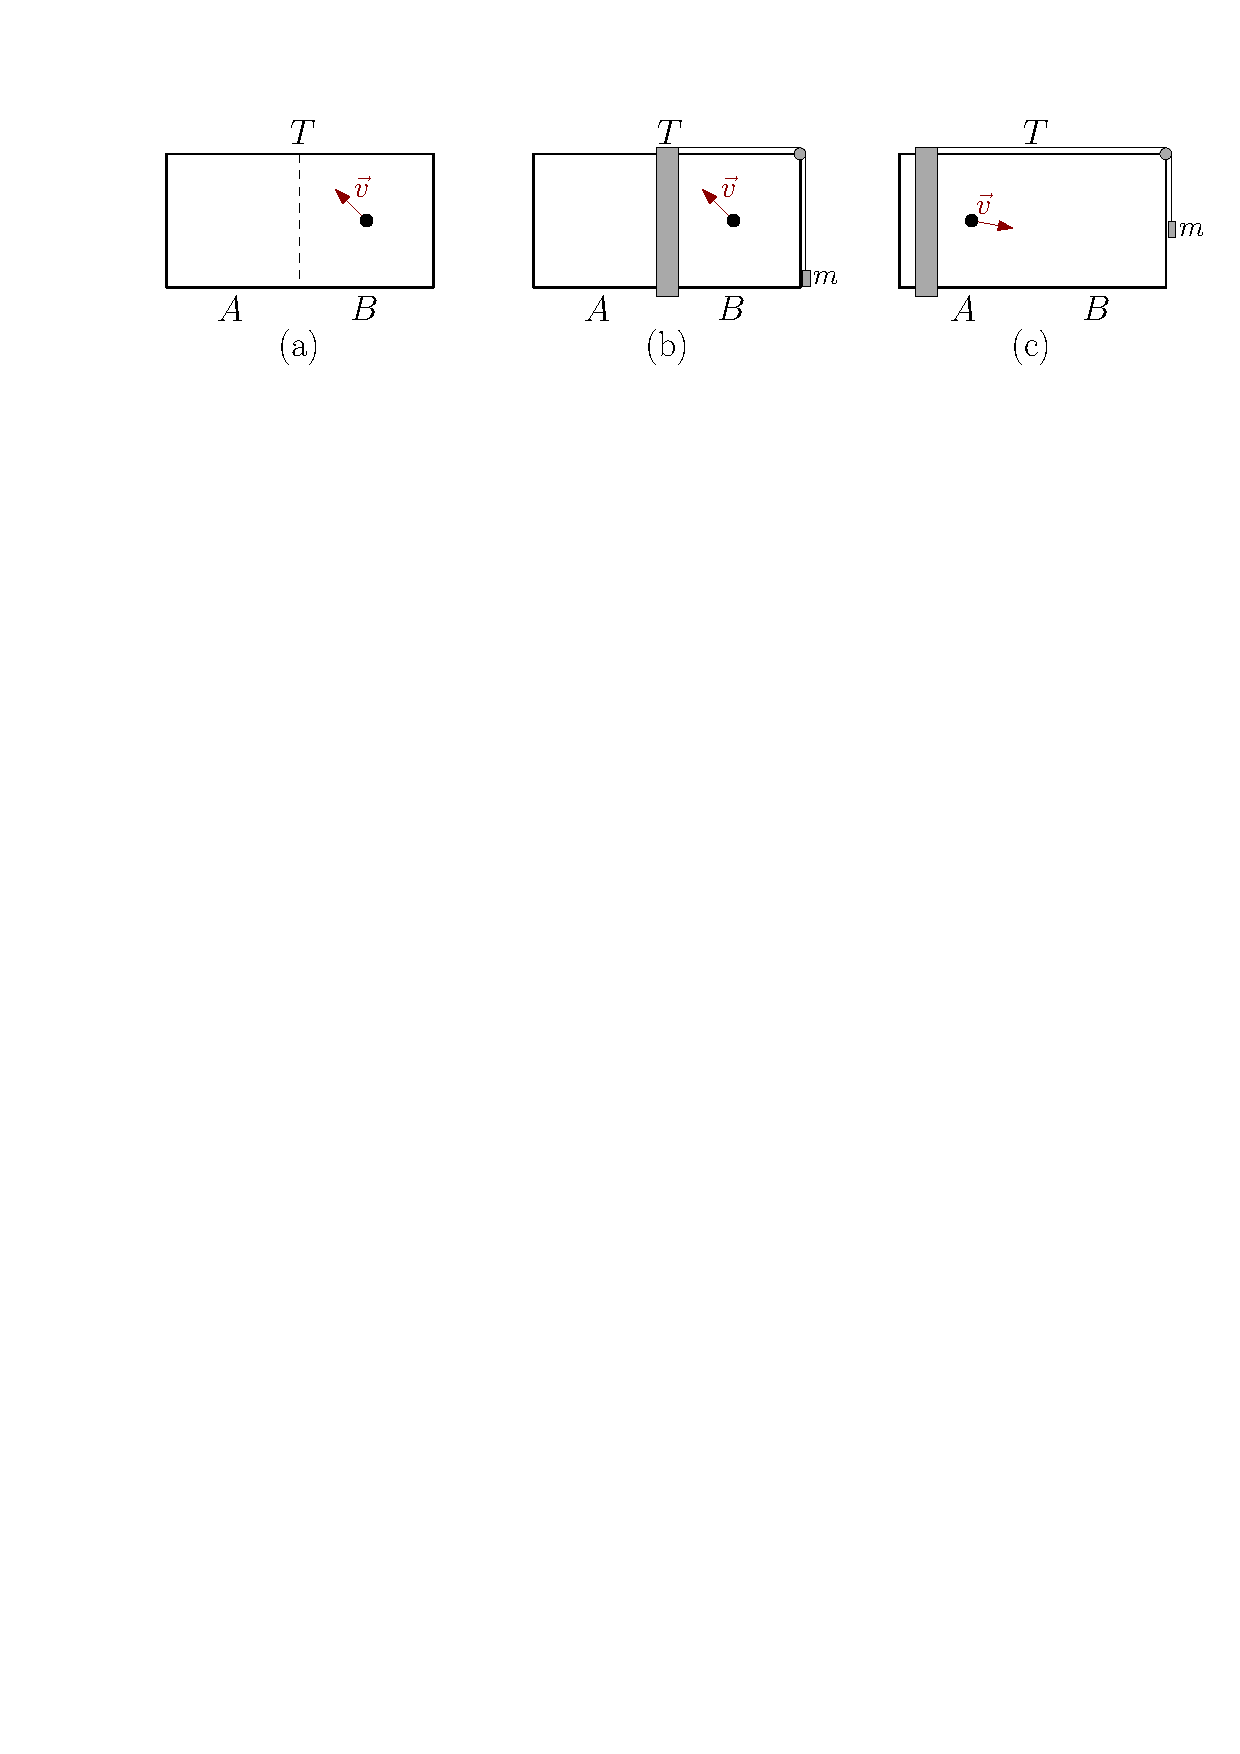
\includegraphics[scale=0.8]{Immagini/27_2/Svilards_engine.pdf}
\caption{Schema del funzionamento del motore di Szilard. In (a) si ha la configurazione iniziale, a temperatura $T$ fissata. Si pone un pistone a dividere $A$ e $B$, e dopo aver misurato la posizione della particella, in (b) si collega una massa $m$ al pistone, dalla parte in cui si trova la particella. In tal modo, in (c) è possibile sfruttare il moto di quest'ultima per fare lavoro. Ipotizzando che il pistone (e carrucola e massa) si muovano senza attrito, il motore ha come unico effetto la produzione di \textit{lavoro} senza alcuna spesa.\label{fig:szilard}}
\end{figure}

Consideriamo in \ref{fig:szilard}.(a) un sistema costituito da due camere comunicanti $A$ e $B$, che si trovano in un bagno termico a temperatura $T$ fissata. Ipotizziamo che vi sia una singola particella $P$, con velocità $\vec{v}$, che effettua urti perfettamente elastici con le pareti del contenitore.\\
Se sappiamo che $P$ si trova in $B$, cioè a destra, possiamo posizionare (in maniera reversibile, senza spendere lavoro) un pistone a separare $A$ e $B$, collegato ad una massa $m$ anch'essa posizionata a \textit{destra} (figura \ref{fig:szilard}.(b)). Prima o poi la particella si scontrerà con la barriera, e potremo quindi estrarre energia da essa (dato che sappiamo in che direzione mettere un \textit{peso} per farlo sollevare dal passaggio, figura \ref{fig:szilard}.(c)).\\
Se la particella si fosse trovata in $A$, cioè a sinistra, avremmo potuto posizionare il peso in maniera simmetrica - di nuovo senza alcuna differenza di energia spesa rispetto al caso precedente - e stavolta sfruttare il movimento di $P$ da sinistra a destra.\\
Ipotizzando che il pistone si muova senza attrito, riposizionarlo non consuma alcuna energia (potremmo pensare ad un sistema di \textit{molle} che consentano di passare reversibilmente da una configurazione all'altra), e perciò abbiamo appena ottenuto una macchina termica che ha come unico effetto quello di generare lavoro, in completa violazione del secondo principio della termodinamica.\\

La situazione si risolve se consideriamo, oltre al sistema di due camere, anche la \textit{memoria} dell'osservatore. Per far funzionare il motore, infatti, abbiamo eseguito una misura di posizione della particella. Ciò, in principio, non crea problema - possiamo pensare che tale misura avvenga in maniera passiva, senza spese - ma presuppone la possibilità di \textbf{registrarne l'esito}, dato che poi dovremo basarci su di esso per posizionare la massa $m$ a destra o a sinistra.\\
Perciò, se vogliamo riportare il motore di Szilard allo stato iniziale, per poi ripetere il ciclo ed estrarre energia, dobbiamo \textit{cancellare} l'esito della misura precedente. Si dà il caso che tale operazione \textbf{consumi per forza energia}.\\

L'idea è data dal \textbf{principio di Landauer}\index{Principio!Landauer}. Consideriamo un registro a $1$ bit in cui \q{salvare} la misura fatta in \ref{fig:szilard}.(a). Tale registro è un \textbf{oggetto fisico}, realizzato con un sistema a due stati, che possiamo immaginare come una camera bipartita da un pistone, con volume $V$ e temperatura $T$ fissati. Vi sono $2$ configurazioni possibili, che corrispondono ai due possibili stati ($0$ o $1$) del bit. Per esempio $0$ potrebbe essere associato alla presenza della particella nella cella a sinistra, e $1$ in quella a destra. Avremo allora un'entropia iniziale $S_i = k_B \log 2$.\\
Per cancellare il bit eliminiamo la divisione, portando a $1$ il numero di stati, e quindi l'entropia $S_f$ a $0$. Abbiamo quindi una variazione $\Delta S = -k_B \log 2$.\\
Applicando allora il secondo principio della termodinamica, si ha che $\Delta S_{tot} = \Delta S_{amb} + \Delta S_{syst} \geq 0$, dove per ambiente intendiamo il bagno a temperatura $T$, mentre la $\Delta S_{syst}$ è stata appena calcolata.\\
Tuttavia, per una riserva termica infinita (perciò sempre all'equilibrio) possiamo usare la formula di Clausius, e quindi:
\begin{align*}
\Delta S_{amb} =\frac{Q_{amb}}{T}
\end{align*}
Ne deriva che \textit{cancellare} il bit richiede uno scambio di calore con la sorgente, e quindi una \textit{dissipazione}:
\begin{align*}
Q_{amb} \geq k_B T \log 2
\end{align*}
Applicando allora il primo principio della termodinamica, affinché l'energia del sistema non cambi (per poter rieseguire il ciclo), si avrà $Q=W$, e perciò la \textit{cancellazione} del bit richiede una \textbf{spesa energetica} che al \textbf{minimo} è: \marginpar{Principio di Landauer}
\begin{align*}
\Delta \mathcal{E} = kT \log 2 
\end{align*}
In altre parole, c'è un limite \textit{minimo} all'energia spesa per una singola computazione \textit{irreversibile} (come la cancellazione di un bit).

\subsection{Definizioni di base}

Possiamo schematizzare un \textbf{computer}\marginpar{Computer}\index{Computer!classico} come un oggetto che dato un \textit{input} (condizione iniziale), costituito da un sistema fisico opportunamente preparato, lo trasforma tramite un \textit{processo fisico} cambiandone lo \textit{stato logico} (ossia le \textit{informazioni} in esso codificate), e generando così un sistema che, una volta misurato, produce un \textit{output} (risultato).\\

Un \textbf{computer quantistico}\index{Computer!quantistico} \marginpar{Computer quantistico} segue lo stesso schema, usando però per gli stati delle \textit{funzioni d'onda}. Avremo quindi uno stato iniziale $\ket{\psi_{in}}$, che subisce un'evoluzione temporale tramite l'operatore $U=\exp\left(-\frac{i}{\hbar}tH\right)$, giungendo ad un output $\ket{\psi_{out}}=U\ket{\psi_{in}}$. Per poterlo usare, tuttavia, dobbiamo effettuare una misura, che selezionerà solo uno dei possibili esiti codificati da $\ket{\psi_{out}}$. Perciò, l'algoritmo quantistico deve far sì che l'esito desiderato possa essere estratto in maniera efficiente dalla funzione d'onda finale, cosa che in genere è un problema complesso.

\begin{figure}[H]
\centering
\tikzset{every picture/.style={line width=0.75pt}} %set default line width to 0.75pt        
\begin{center}
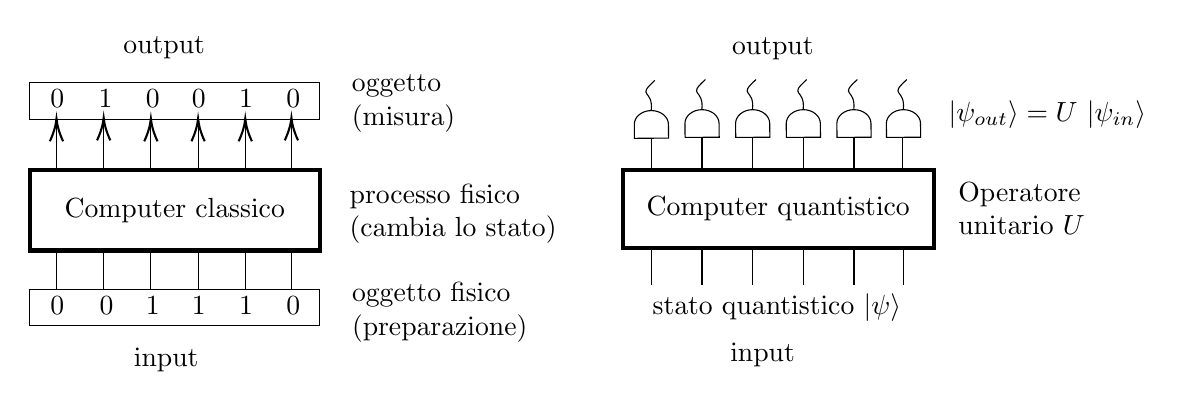
\begin{tikzpicture}[x=0.75pt,y=0.75pt,yscale=-1,xscale=0.97]
%uncomment if require: \path (0,300); %set diagram left start at 0, and has height of 300

%Shape: Rectangle [id:dp3370854768451652] 
\draw  [line width=1.5]  (38.19,137.13) -- (182.22,137.13) -- (182.22,175.83) -- (38.19,175.83) -- cycle ;
%Straight Lines [id:da444794365909732] 
\draw    (51.47,176.17) -- (51.47,194.51) ;


%Straight Lines [id:da3309151478008787] 
\draw    (74.91,175.83) -- (74.91,194.17) ;


%Straight Lines [id:da5291423146743008] 
\draw    (98.35,176.17) -- (98.35,194.51) ;


%Straight Lines [id:da8471848239987096] 
\draw    (121.8,176.17) -- (121.8,194.51) ;


%Straight Lines [id:da5685433525068389] 
\draw    (145.24,176.17) -- (145.24,194.51) ;


%Straight Lines [id:da37769970174090206] 
\draw    (168.16,175.83) -- (168.16,194.17) ;


%Straight Lines [id:da3063143558848054] 
\draw    (51.47,114.31) -- (51.47,136.9) ;

\draw [shift={(51.47,112.31)}, rotate = 90] [color={rgb, 255:red, 0; green, 0; blue, 0 }  ][line width=0.75]    (10.93,-3.29) .. controls (6.95,-1.4) and (3.31,-0.3) .. (0,0) .. controls (3.31,0.3) and (6.95,1.4) .. (10.93,3.29)   ;
%Straight Lines [id:da7551493211306404] 
\draw    (74.91,113.85) -- (74.91,136.44) ;

\draw [shift={(74.91,111.85)}, rotate = 90] [color={rgb, 255:red, 0; green, 0; blue, 0 }  ][line width=0.75]    (10.93,-3.29) .. controls (6.95,-1.4) and (3.31,-0.3) .. (0,0) .. controls (3.31,0.3) and (6.95,1.4) .. (10.93,3.29)   ;
%Straight Lines [id:da8373218927741573] 
\draw    (98.35,114.31) -- (98.35,136.9) ;

\draw [shift={(98.35,112.31)}, rotate = 90] [color={rgb, 255:red, 0; green, 0; blue, 0 }  ][line width=0.75]    (10.93,-3.29) .. controls (6.95,-1.4) and (3.31,-0.3) .. (0,0) .. controls (3.31,0.3) and (6.95,1.4) .. (10.93,3.29)   ;
%Straight Lines [id:da8820817105984171] 
\draw    (121.8,114.31) -- (121.8,136.9) ;

\draw [shift={(121.8,112.31)}, rotate = 90] [color={rgb, 255:red, 0; green, 0; blue, 0 }  ][line width=0.75]    (10.93,-3.29) .. controls (6.95,-1.4) and (3.31,-0.3) .. (0,0) .. controls (3.31,0.3) and (6.95,1.4) .. (10.93,3.29)   ;
%Straight Lines [id:da23173642990564458] 
\draw    (145.24,114.31) -- (145.24,136.9) ;

\draw [shift={(145.24,112.31)}, rotate = 90] [color={rgb, 255:red, 0; green, 0; blue, 0 }  ][line width=0.75]    (10.93,-3.29) .. controls (6.95,-1.4) and (3.31,-0.3) .. (0,0) .. controls (3.31,0.3) and (6.95,1.4) .. (10.93,3.29)   ;
%Straight Lines [id:da3352885240092238] 
\draw    (168.16,113.85) -- (168.16,136.44) ;

\draw [shift={(168.16,111.85)}, rotate = 90] [color={rgb, 255:red, 0; green, 0; blue, 0 }  ][line width=0.75]    (10.93,-3.29) .. controls (6.95,-1.4) and (3.31,-0.3) .. (0,0) .. controls (3.31,0.3) and (6.95,1.4) .. (10.93,3.29)   ;
%Shape: Rectangle [id:dp8501179019878584] 
\draw   (38.19,95) -- (182.22,95) -- (182.22,112.53) -- (38.19,112.53) -- cycle ;
%Shape: Rectangle [id:dp18502125567242067] 
\draw   (38.19,194.51) -- (182.22,194.51) -- (182.22,212.04) -- (38.19,212.04) -- cycle ;
%Shape: Rectangle [id:dp08080369161895873] 
\draw  [line width=1.5]  (332.7,137.23) -- (487.26,137.23) -- (487.26,174.6) -- (332.7,174.6) -- cycle ;
%Straight Lines [id:da5174976099608133] 
\draw    (346.96,174.93) -- (346.96,192.62) ;


%Straight Lines [id:da3906594571053619] 
\draw    (372.11,174.6) -- (372.11,192.29) ;


%Straight Lines [id:da08487629323958013] 
\draw    (397.27,174.93) -- (397.27,192.62) ;


%Straight Lines [id:da6583582327013684] 
\draw    (422.42,174.93) -- (422.42,192.62) ;


%Straight Lines [id:da8933659412949497] 
\draw    (447.57,174.93) -- (447.57,192.62) ;


%Straight Lines [id:da03377065386226974] 
\draw    (472.17,174.6) -- (472.17,192.29) ;


%Straight Lines [id:da7845188854936893] 
\draw    (346.96,121.69) -- (346.96,137.01) ;


%Straight Lines [id:da5758058639542603] 
\draw    (372.11,121.4) -- (372.11,136.73) ;


%Straight Lines [id:da8825945599217435] 
\draw    (397.27,121.69) -- (397.27,137.01) ;


%Straight Lines [id:da027631106900613434] 
\draw    (422.42,121.69) -- (422.42,137.01) ;


%Straight Lines [id:da9616245238371959] 
\draw    (447.57,121.69) -- (447.57,137.01) ;


%Straight Lines [id:da6887376007663764] 
\draw    (471.89,121.69) -- (471.89,137.01) ;


%Flowchart: Delay [id:dp748952144669494] 
\draw   (338.54,121.81) -- (338.47,115.15) .. controls (338.43,111.48) and (342.19,108.47) .. (346.87,108.44) .. controls (351.55,108.41) and (355.38,111.37) .. (355.42,115.04) -- (355.49,121.7) -- cycle ;
%Flowchart: Delay [id:dp3966652317655148] 
\draw   (363.69,121.37) -- (363.62,114.71) .. controls (363.58,111.04) and (367.35,108.03) .. (372.03,108) .. controls (376.71,107.97) and (380.53,110.93) .. (380.57,114.61) -- (380.64,121.27) -- cycle ;
%Flowchart: Delay [id:dp8688199158082022] 
\draw   (388.85,121.37) -- (388.78,114.71) .. controls (388.74,111.04) and (392.5,108.03) .. (397.18,108) .. controls (401.86,107.97) and (405.69,110.93) .. (405.72,114.61) -- (405.8,121.27) -- cycle ;
%Flowchart: Delay [id:dp8086320640430136] 
\draw   (414,121.37) -- (413.93,114.71) .. controls (413.89,111.04) and (417.65,108.03) .. (422.33,108) .. controls (427.01,107.97) and (430.84,110.93) .. (430.88,114.61) -- (430.95,121.27) -- cycle ;
%Flowchart: Delay [id:dp722358729241092] 
\draw   (439.16,121.37) -- (439.08,114.71) .. controls (439.05,111.04) and (442.81,108.03) .. (447.49,108) .. controls (452.17,107.97) and (455.99,110.93) .. (456.03,114.61) -- (456.1,121.27) -- cycle ;
%Flowchart: Delay [id:dp16472187429517238] 
\draw   (463.75,121.37) -- (463.68,114.71) .. controls (463.64,111.04) and (467.4,108.03) .. (472.08,108) .. controls (476.76,107.97) and (480.59,110.93) .. (480.63,114.61) -- (480.7,121.27) -- cycle ;
%Curve Lines [id:da02121963440081065] 
\draw    (373.79,93.49) .. controls (364.29,101.84) and (373.23,97.44) .. (372.03,108) ;


%Curve Lines [id:da31983882752062054] 
\draw    (348.64,93.93) .. controls (339.13,102.28) and (348.08,97.88) .. (346.87,108.44) ;


%Curve Lines [id:da4623293987746533] 
\draw    (398.94,93.49) .. controls (389.44,101.84) and (398.38,97.44) .. (397.18,108) ;


%Curve Lines [id:da5783366480443313] 
\draw    (424.1,93.49) .. controls (414.59,101.84) and (423.54,97.44) .. (422.33,108) ;


%Curve Lines [id:da4188892016494363] 
\draw    (449.25,93.49) .. controls (439.75,101.84) and (448.69,97.44) .. (447.49,108) ;


%Curve Lines [id:da14876622747392365] 
\draw    (473.84,93.49) .. controls (464.34,101.84) and (473.28,97.44) .. (472.08,108) ;



% Text Node
\draw (110.2,156.48) node  [align=left] {Computer classico};
% Text Node
\draw (51.86,102.86) node   {$0$};
% Text Node
\draw (75.82,102.86) node   {$1$};
% Text Node
\draw (99.27,102.86) node   {$0$};
% Text Node
\draw (122.19,102.86) node   {$0$};
% Text Node
\draw (145.63,102.86) node   {$1$};
% Text Node
\draw (169.07,102.86) node   {$0$};
% Text Node
\draw (51.86,202.36) node   {$0$};
% Text Node
\draw (76.34,202.36) node   {$0$};
% Text Node
\draw (99.27,202.36) node   {$1$};
% Text Node
\draw (122.19,202.36) node   {$1$};
% Text Node
\draw (145.63,202.36) node   {$1$};
% Text Node
\draw (169.07,202.36) node   {$0$};
% Text Node
\draw (105.93,228.61) node  [align=left] {input};
% Text Node
\draw (104.97,78.34) node  [align=left] {output};
% Text Node
\draw (241.82,205.7) node  [align=left] {oggetto fisico\\(preparazione)};
% Text Node
\draw (248.47,158.25) node  [align=left] {processo fisico\\(cambia lo stato)};
% Text Node
\draw (223.87,104.97) node  [align=left] {oggetto\\(misura)};
% Text Node
\draw (409.98,155.91) node  [align=left] {Computer quantistico};
% Text Node
\draw (402.17,226.25) node  [align=left] {input};
% Text Node
\draw (407.28,78.58) node  [align=left] {output};
% Text Node
\draw (409.28,203.17) node  [align=left] {stato quantistico $\displaystyle |\psi \rangle $};
% Text Node
\draw (530.86,155.69) node  [align=left] {Operatore\\unitario $\displaystyle U$};
% Text Node
\draw (532.54,110.19) node  [align=left] {$ $};
% Text Node
\draw (545.95,110.19) node   {$|\psi _{out} \rangle =U\ |\psi _{in} \rangle \ $};


\end{tikzpicture}
\end{center}
\caption{Schema a blocchi di un computer classico o quantistico\label{fig:computer-classico-quantistico}}
\end{figure}

Tuttavia, nel processo fisico possiamo usare tutte le possibilità offerte dalla \MQ, come l'\textit{entanglement}, il \textit{principio di sovrapposizione}, il \textit{teletrasporto}... con una \textbf{grave limitazione}:\marginpar{No cloning theorem} non è possibile creare una copia esatta di uno stato senza distruggere l'originale (\textbf{no cloning theorem}).\\

Strettamente collegato al concetto di \textbf{computazione} si trova l'idea di \textbf{comunicazione}.\\

Per \textbf{comunicazione classica}\index{Comunicazione!classica} si intende il trasferimento di informazione da un mittente (\textbf{A}lice) e un destinatario (\textbf{B}ob), attraverso un determinato \textbf{canale}. Ciò è realizzato tramite un sistema in grado di trasferire \textit{bit} di informazione (dato che un qualsiasi stato logico classico può essere scritto come un'opportuna sequenza di $0$ e $1$).\\

Nuovamente, la \textbf{comunicazione quantistica}\index{Comunicazione!quantistica} segue lo stesso schema, ma questa volta si trasferisce una funzione d'onda $\ket{\psi}$ tramite un \textbf{canale quantistico}, per esempio attraverso \textit{fotoni}. La maggiore libertà offerta della \MQ offre possibilità più ampie rispetto a quelle permesse dalla \MC, come la \textit{crittografia quantistica}, il \textit{trasporto di più informazione di quella classicamente permessa}, il \textit{teletrasporto quantistico}...

\begin{figure}[H]
\centering
\tikzset{every picture/.style={line width=0.75pt}} %set default line width to 0.75pt        
\begin{center}
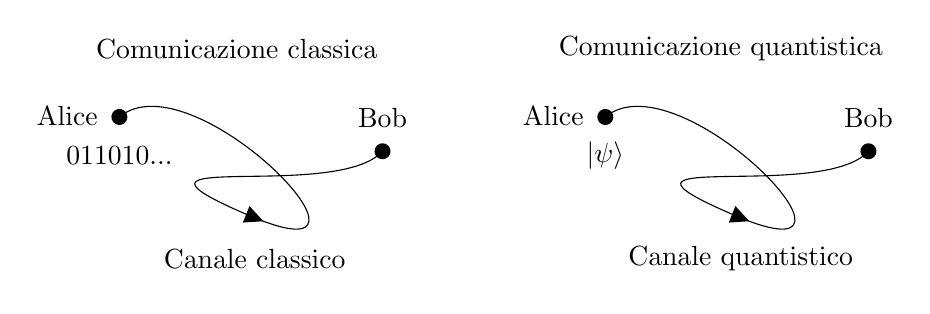
\begin{tikzpicture}[x=0.75pt,y=0.75pt,yscale=-1,xscale=1]
%uncomment if require: \path (0,300); %set diagram left start at 0, and has height of 300

%Curve Lines [id:da4010158625664151] 
\draw    (82.21,107.65) .. controls (118.09,77.9) and (223.93,188.97) .. (145,155.25) .. controls (66.06,121.53) and (186.56,148.97) .. (208.98,124.18) ;
\draw [shift={(208.98,124.18)}, rotate = 312.13] [color={rgb, 255:red, 0; green, 0; blue, 0 }  ][fill={rgb, 255:red, 0; green, 0; blue, 0 }  ][line width=0.75]      (0, 0) circle [x radius= 3.35, y radius= 3.35]   ;
\draw [shift={(82.21,107.65)}, rotate = 320.34] [color={rgb, 255:red, 0; green, 0; blue, 0 }  ][fill={rgb, 255:red, 0; green, 0; blue, 0 }  ][line width=0.75]      (0, 0) circle [x radius= 3.35, y radius= 3.35]   ;
%Straight Lines [id:da260269707512071] 
\draw    (149.72,157.15) -- (145,155.25) ;

\draw [shift={(151.58,157.89)}, rotate = 201.9] [fill={rgb, 255:red, 0; green, 0; blue, 0 }  ][line width=0.75]  [draw opacity=0] (8.93,-4.29) -- (0,0) -- (8.93,4.29) -- cycle    ;
%Curve Lines [id:da24217790755113677] 
\draw    (316.32,107.65) .. controls (352.2,77.9) and (458.05,188.97) .. (379.11,155.25) .. controls (300.18,121.53) and (420.67,148.97) .. (443.1,124.18) ;
\draw [shift={(443.1,124.18)}, rotate = 312.13] [color={rgb, 255:red, 0; green, 0; blue, 0 }  ][fill={rgb, 255:red, 0; green, 0; blue, 0 }  ][line width=0.75]      (0, 0) circle [x radius= 3.35, y radius= 3.35]   ;
\draw [shift={(316.32,107.65)}, rotate = 320.34] [color={rgb, 255:red, 0; green, 0; blue, 0 }  ][fill={rgb, 255:red, 0; green, 0; blue, 0 }  ][line width=0.75]      (0, 0) circle [x radius= 3.35, y radius= 3.35]   ;
%Straight Lines [id:da9217932977595515] 
\draw    (383.83,157.15) -- (379.11,155.25) ;

\draw [shift={(385.69,157.89)}, rotate = 201.9] [fill={rgb, 255:red, 0; green, 0; blue, 0 }  ][line width=0.75]  [draw opacity=0] (8.93,-4.29) -- (0,0) -- (8.93,4.29) -- cycle    ;

% Text Node
\draw (138.72,74.93) node  [align=left] {Comunicazione classica};
% Text Node
\draw (371.94,74.93) node  [align=left] {Comunicazione quantistica};
% Text Node
\draw (57.09,107.32) node  [align=left] {Alice};
% Text Node
\draw (208.98,107.98) node  [align=left] {Bob};
% Text Node
\draw (147.39,176.08) node  [align=left] {Canale classico};
% Text Node
\draw (82.21,126.49) node   {$011010...$};
% Text Node
\draw (291.21,107.32) node  [align=left] {Alice};
% Text Node
\draw (443.1,107.98) node  [align=left] {Bob};
% Text Node
\draw (381.5,176.08) node  [align=left] {Canale quantistico};
% Text Node
\draw (316.32,126.49) node   {$|\psi \rangle $};


\end{tikzpicture}
\end{center}
\caption{Schema di una comunicazione classica o quantistica\label{fig:comunicazione-classica-quantistica}}
\end{figure}

Tramite \textbf{sensori quantistici} è possibile poi effettuare misure con target ben \textit{più piccoli}, superando i limiti delle ampie medie temporali propri dei sensori classici.

\begin{comment}
\section{Gli argomenti che tratteremo}
Tra gli argomenti che affronteremo nel corso vi sono:
\begin{itemize}
\item Qubit, Matrice densità, correlazioni quantistiche, effetto Zeno, Metodo variazionale
\item Software quantistico
\item Teletrasporto, crittografia, comunicazione quantistica, algoritm (Shor, Grover...), simulazioni e sensori
\item Hardware quantistico, panoramica di possibili implementazioni quantistiche (fotoni, superconduttori, atomi freddi, ioni intrappolati, difetti colorati in diamanti...)
\end{itemize}
\end{comment}

\section{Modello di calcolo a circuiti}
\subsection{Calcolo classico deterministico}
Il modello di calcolo comunemente utilizzato nei computer si basa sul computare funzioni da $n$-bit a $m$-bit:
\begin{align}
f: \{0,1\}^n \mapsto \{0,1\}^m
\label{eqn:f-binaria}
\end{align}
dove $0$ e $1$ sono rappresentati come \textbf{stati distinguibili} di un opportuno sistema classico.\\
Una computazione è schematizzata da \textit{linee} che codificano lo stato di un \textit{bit}, su cui si opera tramite \textbf{porte logiche}\index{Porte logiche}. 
\begin{figure}[H]
\centering
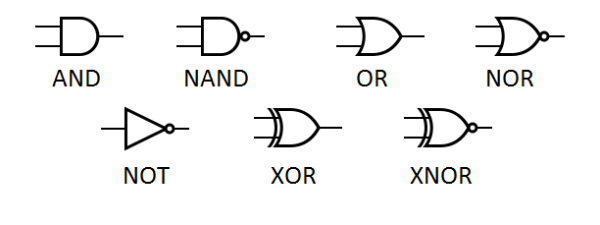
\includegraphics[scale=0.5]{Immagini/27_2/image001.png}
\caption{Schemi delle principali porte logiche\label{fig:porte-logiche}}
\end{figure}
Si può dimostrare che qualsiasi computazione del tipo (\ref{eqn:f-binaria}) può essere realizzata come una combinazione di alcune \textbf{porte logiche fondamentali}, che ora specifichiamo.\\

Partiamo dalle {porte logiche} a \textbf{1 bit}. In tal caso abbiamo due sole possibilità: \textit{identità} e \textit{not}.\index{Porte logiche!1-bit classiche}

\begin{table}[H]
\centering
\begin{tabular}{@{}ll|ll@{}}
\toprule
\multicolumn{2}{c|}{\textbf{Buffer}} & \multicolumn{2}{c|}{\textbf{Not}} \\ \midrule
\multicolumn{1}{c}{$a$} & \multicolumn{1}{c|}{$a$} & \multicolumn{1}{c}{$a$} & \multicolumn{1}{c}{$\bar{a}$} \\
0 & 0 & 0 & 1 \\
1 & 1 & 1 & 0 \\ \bottomrule
\end{tabular}
\caption{Tabella di verità per \textit{not} ($\bar{a}$) e \textit{identità} (buffer)}
\label{tab:notbuffer}
\end{table}

D'altro canto, le porte logiche fondamentali a \textbf{2 bit} sono \textit{and} e \textit{or}.\index{Porte logiche!2-bit classiche}
\begin{table}[H]
\centering
\begin{tabular}{@{}ll|lll@{}}
\toprule
\multicolumn{1}{c}{a} & \multicolumn{1}{c}{b} & \multicolumn{1}{c}{$\land$} & \multicolumn{1}{c}{$\lor$} & \multicolumn{1}{c}{$\otimes$} \\ \midrule
0 & 0 & 0 & 0 & 0 \\
0 & 1 & 0 & 1 & 1 \\
1 & 0 & 0 & 1 & 1 \\
1 & 1 & 1 & 1 & 0 \\ \bottomrule
\end{tabular}
\caption{Tabella di verità per \textit{and} $a \land b = ab$, \textit{or} $a\lor b =a+b$ e \textit{xor} $a\otimes b$}
\label{tab:orandxor}
\end{table}

Due altre possibili operazioni sono il \emph{copy} (copiare l'informazione) e lo \emph{swap} (lo scambio di due stati):

\begin{figure}[H]
\centering
\tikzset{every picture/.style={line width=0.75pt}} %set default line width to 0.75pt        
\begin{center}
\begin{tikzpicture}[x=0.75pt,y=0.75pt,yscale=-1,xscale=1]
%uncomment if require: \path (0,300); %set diagram left start at 0, and has height of 300

%Straight Lines [id:da016426433289817854] 
\draw    (84.92,113.6) -- (124.11,113.47) ;


%Straight Lines [id:da3658468280540397] 
\draw    (124.11,113.47) -- (143.48,88.34) ;


%Straight Lines [id:da7433164045904939] 
\draw    (143.91,138.05) -- (124.11,113.47) ;


%Straight Lines [id:da3375002697884233] 
\draw    (143.48,88.34) -- (182.67,88.2) ;


%Straight Lines [id:da7979080776301537] 
\draw    (143.91,138.05) -- (183.1,137.91) ;


%Straight Lines [id:da5463454905207172] 
\draw    (343.6,112.65) -- (362.98,87.52) ;


%Straight Lines [id:da5313174710619584] 
\draw    (363.41,137.23) -- (343.6,112.65) ;


%Straight Lines [id:da7258415514837049] 
\draw    (362.98,87.52) -- (402.16,87.38) ;


%Straight Lines [id:da047659355452852825] 
\draw    (363.41,137.23) -- (402.59,137.1) ;


%Straight Lines [id:da13818952805033047] 
\draw    (343.6,112.65) -- (323.79,88.06) ;


%Straight Lines [id:da6049009718842897] 
\draw    (324.22,137.78) -- (343.6,112.65) ;


%Straight Lines [id:da2165705811529799] 
\draw    (284.61,88.2) -- (323.79,88.06) ;


%Straight Lines [id:da18208228564131046] 
\draw    (285.04,137.91) -- (324.22,137.78) ;



% Text Node
\draw (76.85,111.02) node   {$a$};
% Text Node
\draw (193.08,84.68) node   {$a$};
% Text Node
\draw (192.89,134.52) node   {$a$};
% Text Node
\draw (412.81,85.19) node   {$b$};
% Text Node
\draw (413.05,134.36) node   {$a$};
% Text Node
\draw (275.01,86.17) node   {$a$};
% Text Node
\draw (276.34,136) node   {$b$};
% Text Node
\draw (131.34,164.53) node  [align=left] {copy};
% Text Node
\draw (345.11,165.62) node  [align=left] {swap};


\end{tikzpicture}
\end{center}
\caption{Schema del funzionamento delle porte logiche \textbf{copy} e \textbf{swap}\label{fig:copy-swap}}
\end{figure}

Un \textit{set uiniversale classico}, ossia l'insieme di operazioni logiche necessarie per eseguire una computazione logica generica, è dato da \textit{and}, \textit{or}, \textit{not}, \textit{copy}. Si può dimostrare che un set \textbf{minimale} è costituito da \textit{copy} e una scelta tra \textit{nand} e \textit{nor} \cite{nand2tetris}.\\

Notiamo che alcune di queste operazioni sono \textbf{irreversibili}\marginpar{Irreversibilità delle porte logiche classiche}, cioè dallo stato finale non è possibile risalire con univocità allo stato iniziale (es. per \textit{or} e \textit{and} input e output non sono in relazione biunivoca). Ciò è problematico, perché la \MQ agisce in maniera unitaria e reversibile, e quindi di certo non è possibile trovare le \textit{porte logiche quantistiche} per semplice trasposizione. Inoltre, come già accennato, non è possibile effettuare l'operazione di \textit{copy} in \MQ.

\subsection{Calcolo quantistico}
L'analogo quantistico di un bit classico è detto \textbf{qubit}, per cui si intende un set di due possibili stati (quantistici) distinguibili: \textit{fondamentale} $\ket{0}$ ed \textit{eccitato} $\ket{1}$.

\begin{figure}[H]
\centering


\tikzset{every picture/.style={line width=0.75pt}} %set default line width to 0.75pt        
\begin{center}
\begin{tikzpicture}[x=0.75pt,y=0.75pt,yscale=-1,xscale=1]
%uncomment if require: \path (0,300); %set diagram left start at 0, and has height of 300

%Straight Lines [id:da35494731744920616] 
\draw    (180.08,120.33) -- (270.58,120.33) ;


%Straight Lines [id:da8080577379615441] 
\draw    (180.5,160) -- (270.25,160) ;



% Text Node
\draw (286,118.5) node   {$|0\rangle $};
% Text Node
\draw (285.5,159) node   {$|1\rangle $};


\end{tikzpicture}
\end{center}
\caption{Come nel caso classico, rappresentiamo i \textit{qubit} come linee, che saranno opportunamente collegate agli input delle porte logiche\label{fig:qubit-righe}}
\end{figure}

Dal principio di sovrapposizione della \MQ deriva immediatamente la possibilità di creare stati \textit{senza analogo classico}. Infatti, un generico qubit è dato da una \textbf{superposizione} dei due stati possibili:
\begin{align*}
\ket{\psi} = \alpha_0 \ket{0} + \alpha_1 \ket{1} \qquad \alpha_0, \alpha_1 \in \bb{C}, |\alpha_0|^2 + |\alpha_1|^2 = 1
\end{align*}
Equivalentemente, riscrivendo $\alpha_0$ e $\alpha_1$ come fasi, otteniamo l'espressione:
\begin{align*}
\ket{\psi} = \cos\frac{\theta}{2} \ket{0} + \sin\frac{\theta}{2} e^{i\varphi} \ket{1} \qquad 0\leq \theta \leq \pi, 0 \leq \varphi \leq \pi
\end{align*}

Tale espressione ha un'interpretazione geometrica come un \textbf{vettore unitario} nella \textbf{sfera di Bloch}\index{Sfera di Bloch} (figura \ref{fig:blochsphere}).

\begin{figure}[H]
\centering
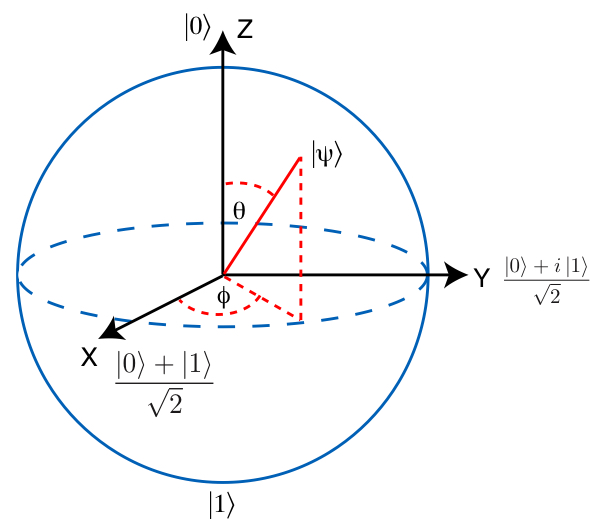
\includegraphics[scale=0.4]{Immagini/27_2/image002.png}
\caption{Rappresentazione grafica della \textbf{sfera di Bloch}\label{fig:blochsphere}}
\end{figure}
\end{document}
